\subsection{Deep Neural Network}
\label{sec:dnn}

\begin{figure}[t]
	\centering
	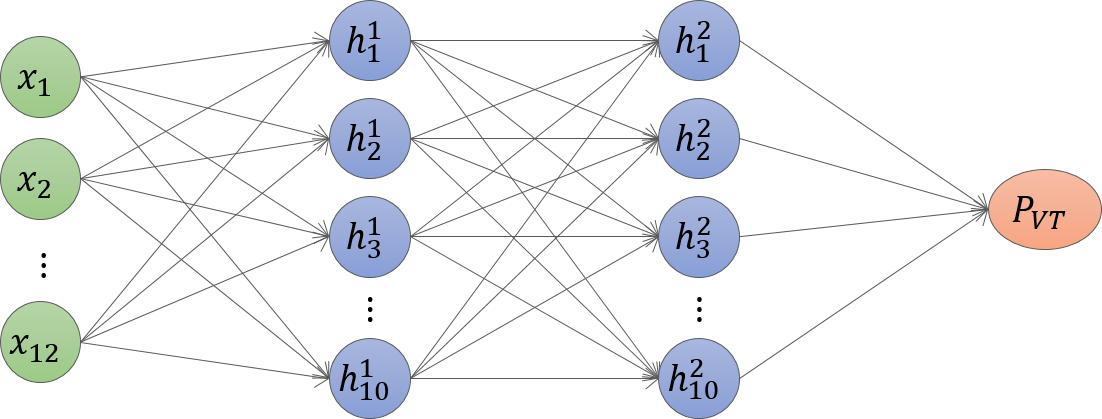
\includegraphics[width=0.5\textwidth]{figures/dnn_graph.png}
	\caption{DNN architecture}
	\label{fig:dnn_graph}
\end{figure}

The proposed DNN model consists of 2 hidden layers with 10 neurons 
each $12$ 
neurons in the input layer and one node in the output layer, see 
Figure~\ref{fig:dnn_graph}.
Relu activation functions are used, output layer uses logistic 
sigmoid activation function to produce an estimate of the probability 
of VT label.
At the training phase we minimize the cross-entropy loss 
$l_{\log}:\{0,1\}\times[0,1]\rightarrow\mathbb{R}_{+}$:
\begin{equation}
l_{\log}(y,p)= -y\log p - (1-y)\log(1-p)
\end{equation}

